\section{Data Requirements Analysis and Description}
\subsection{Research Related Applications/Systems for Reference}
\subsubsection{Rationale for choosing Steam as the primary reference system
}
Steam was selected as the primary reference system because it closely matches the scope of the proposed application. Rather than functioning only as an online game store, Steam operates as an integrated digital distribution platform that combines user accounts, storefront browsing, purchasing, personal library management, and community interaction. This makes it highly relevant as a reference for a system that must support both commercial transactions and long-term user engagement.

\begin{figure}[h!]
    \centering
    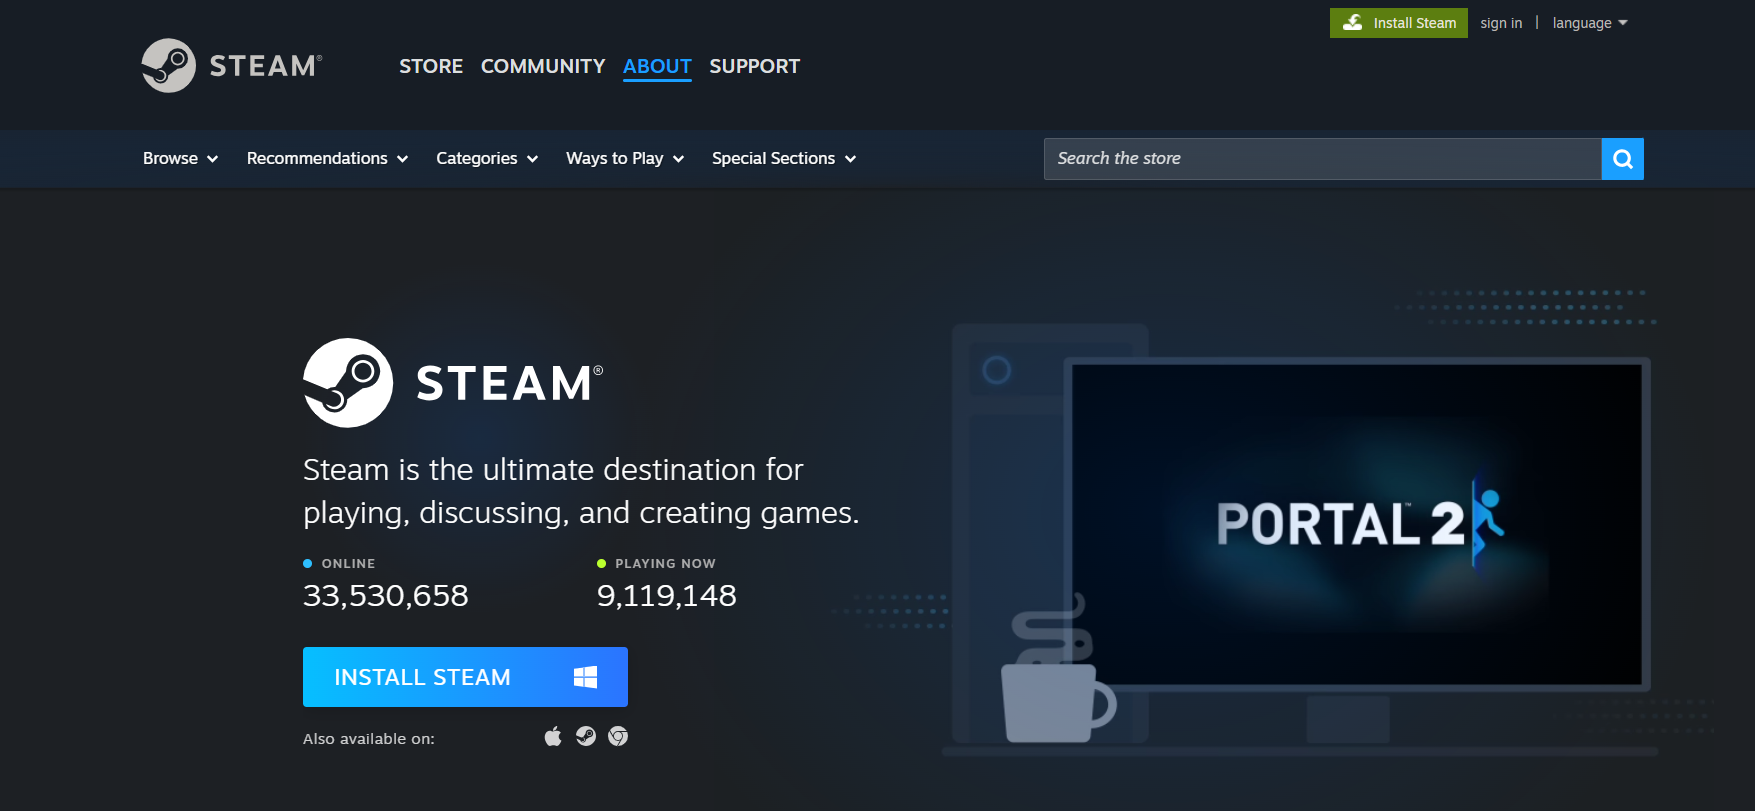
\includegraphics[width=0.75\linewidth]{graphics/fig2.png}
    \caption{Steam platform overview page}
    \label{fig:steam_overview}
\end{figure}
\\
\textit{ The interface illustrates that Steam functions as an integrated digital distribution and community platform rather than a standalone online storefront. This makes it a suitable primary reference system for the proposed system.}
\subsubsection{Scope of Observation and Survey Approach}
The group surveyed Steam from a data-oriented and system-analysis perspective rather than treating it solely as an end-user application. The purpose of this survey was to identify the types of data, user actions, and business relationships reflected in the platform’s interface structure, displayed content, and interaction flows.

The scope of observation focused on the main areas of Steam that are directly relevant to the proposed system, including user account interfaces, storefront navigation, game detail pages, cart and checkout processes, personal library management, achievement tracking, reviews, and community-related features. In addition, the group also observed evidence of developer/publisher involvement through product page information such as publisher details, downloadable content (DLC), pricing, and promotional structures.
User Management and Account-Based Access
Each observed element was treated as a basis for inferring data storage requirements, entity types, attributes, relationships, and business rules. As a result, the proposed system is grounded in a real-world platform that can be clearly observed and systematically analyzed.
\subsubsection{Business Analysis of Steam in Relation to the Proposed System}
This section should analyze \textbf{how Steam operates as a real-world information system}, \textbf{what business processes can be observed from it}, and \textbf{why those processes provide a suitable foundation for the proposed system.} Instead of merely listing features, the section should explain how Steam supports content distribution, purchasing, ownership management, community interaction, and publisher-side participation.
\paragraph{User Management and Account-Based Access}
Steam operates as a digital platform built around user accounts, in which most core activities are tied to a persistent user identity. To access personalized services, users must sign in with their account credentials or use alternative authentication methods such as QR-based login. This shows that account management is a fundamental business function of the platform rather than merely a supporting feature.

From a business perspective, account-based access enables Steam to provide secure and personalized services. In particular, a signed-in user can:
\begin{itemize}
    \item purchase digital products through the platform
    \item access and manage a personal game library
    \item maintain a personal profile
    \item submit reviews and other user-generated content
    \item track achievement progress
    \item interact with community and social features
\end{itemize}

The login interface also suggests the existence of several authentication-related data elements, including:
\begin{itemize}
    \item account name
    \item password credentials
    \item session persistence
    \item account recovery support
\end{itemize}

In addition, Steam's account-centered structure implies that the platform must support multiple types of users with different interaction purposes. While players use their accounts to consume content and participate in the community, the broader structure of the platform also reflects the participation of developer/publisher-side users through product and publishing activities. Therefore, account management is significant not only for authentication, but also for enabling role-based interaction across the platform.
\begin{figure}[h!]
    \centering
    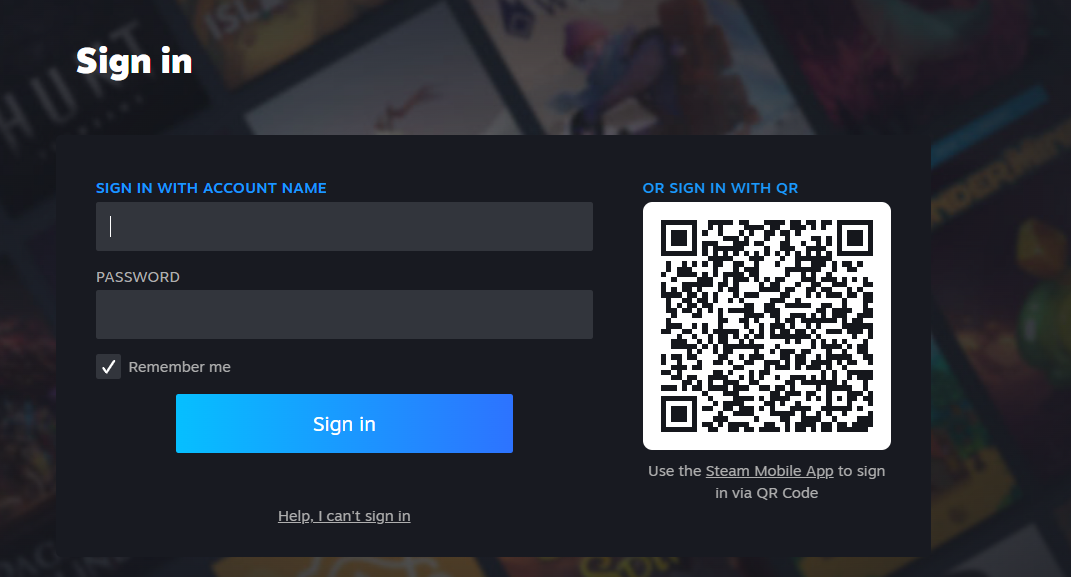
\includegraphics[width=0.75\linewidth]{graphics/loginsteam.png}
    \caption{Steam sign-in interface}
    \label{fig:steam_overview}
\end{figure}

\textit{This interface indicates that Steam relies on account-based access to connect each user with personalized platform activities, including transactions, owned content, and social interaction.}
\paragraph{Digital Product Presentation and Content Discovery}
Steam functions not only as a platform for selling digital games, but also as a structured environment for presenting and organizing game content in ways that support discovery and purchase decisions. Through its storefront, users can browse games by category, genre, tag, recommendation, popularity, or promotional event. This shows that the platform must manage a large amount of descriptive and classificatory information in order to help users navigate a broad digital catalog efficiently. From a business perspective, this function is essential because it connects available products with user interest and directly influences purchasing behavior.

Each game page on Steam presents multiple layers of information beyond the game title itself. These typically include:
\begin{itemize}
    \item price
    \item release date
    \item developer
    \item publisher
    \item descriptive text
    \item screenshots and trailers
    \item tags and genres
    \item system requirements.
\end{itemize}

Such presentation indicates that a game on Steam is treated as a complex digital product rather than a simple item for sale. In addition, these data elements help users evaluate whether a game matches their preferences and technical conditions before making a purchase. Therefore, the storefront is not merely a visual interface, but a business mechanism for organizing product data and supporting content discovery.

From a system analysis perspective, this observed structure provides a clear basis for later data modeling in the proposed system. In particular, it suggests the need for:
\begin{itemize}
    \item entities related to games,
    \item classification mechanisms such as genres and tags,
    \item developer/publisher associations, and
    \item product presentation attributes.
\end{itemize}

As a result, Steam serves as a strong reference for understanding how digital products should be structured, displayed, and connected to user-facing discovery functions in the proposed platform.
\begin{figure}[h!]
    \centering
    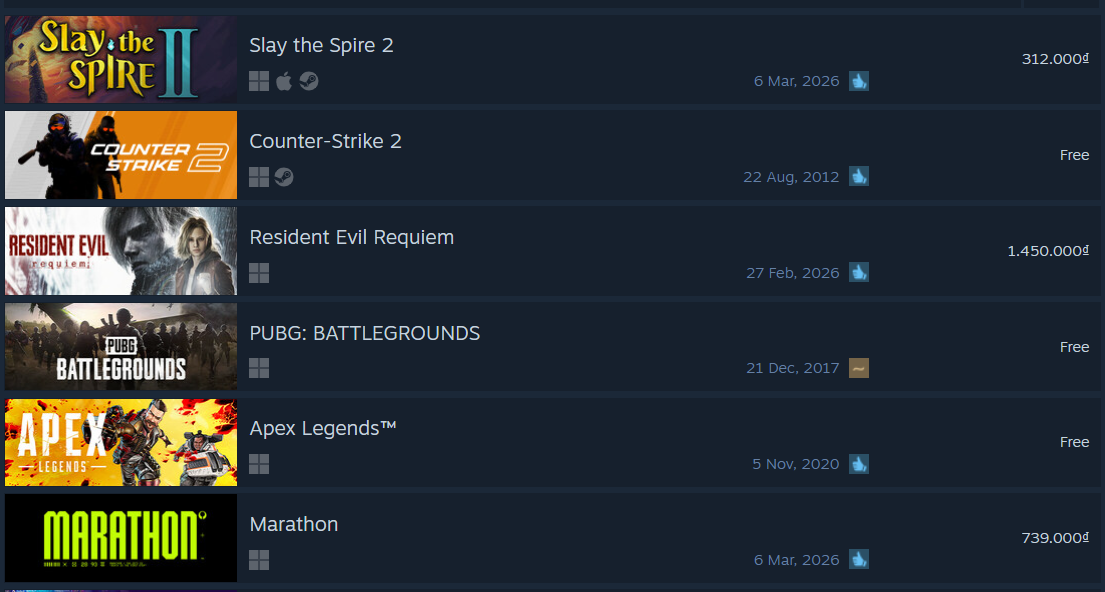
\includegraphics[width=0.6\linewidth]{graphics/steam.png}
    \caption{Steam storefront browsing interface}
    \label{fig:steam_overview}
    
    \vspace{0.5em}
    {\raggedright
    \textit{The Steam storefront organizes digital products through structured listing information such as titles, release dates, and prices, thereby supporting content discovery and user browsing behavior.}
    \par}
\end{figure}

\begin{figure}[h!]
    \centering
    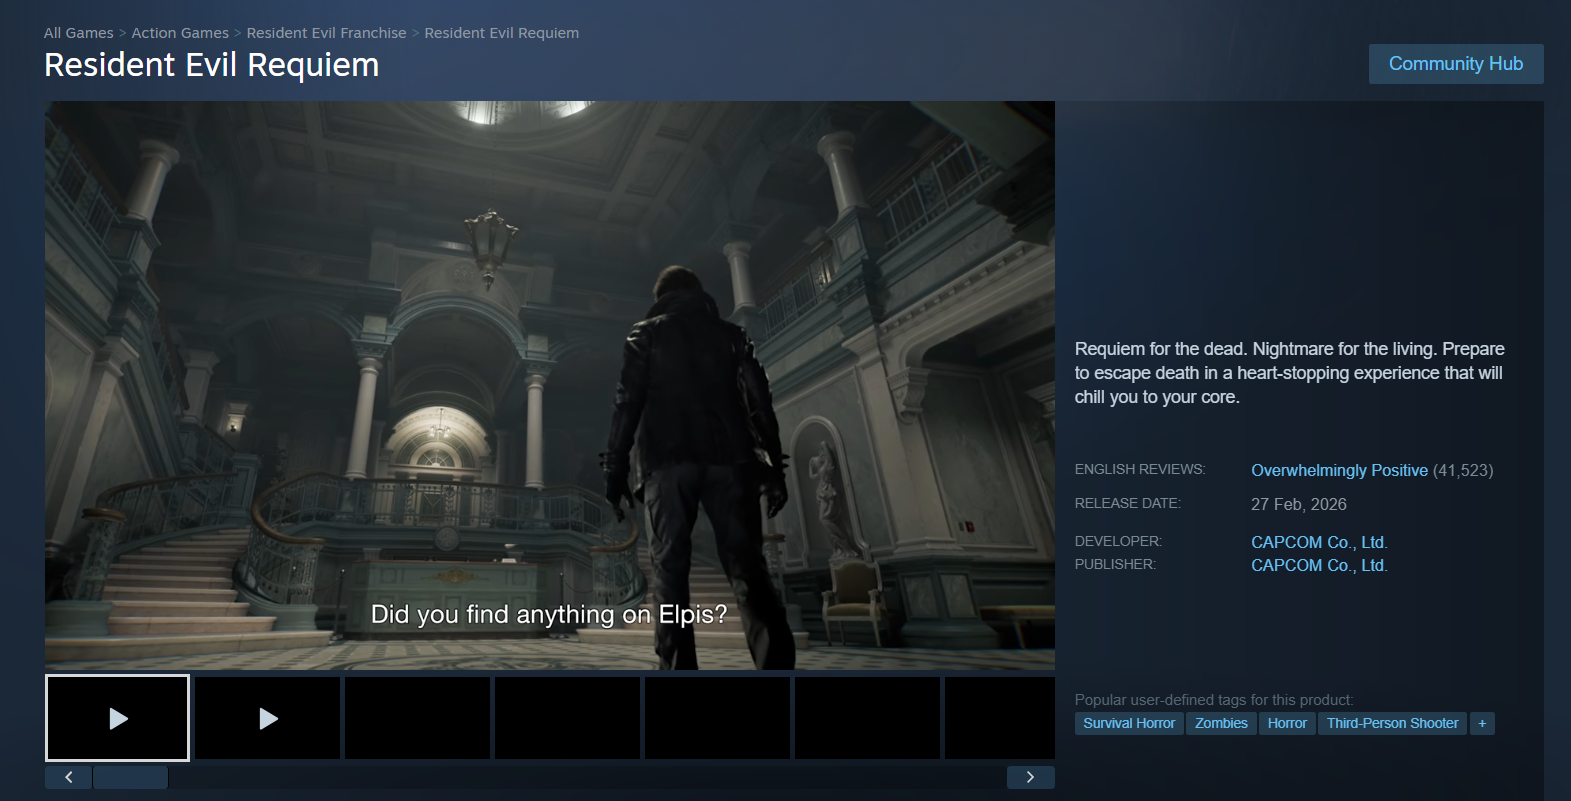
\includegraphics[width=0.6\linewidth]{graphics/steam2.png}
    \caption{Steam game detail page}
    \label{fig:steam_detail}
    
    \vspace{0.5em}
    {\raggedright
    \textit{The Steam game detail interface illustrates that a digital product is represented through multiple layers of information, such as media presentation, review indicators, release information, developer/publisher details, and tags, thereby supporting structured content discovery and purchase consideration.}
    \par}
\end{figure}
\newpage
\newpage
\paragraph{Cart, Checkout, and Transaction Processing}
Steam also demonstrates a complete digital purchasing workflow in which a player can select products, place them in a shopping cart, and proceed to checkout before a purchase is finalized. This shows that the platform does not treat purchasing as a single instant action, but as a multi-step business process.

From a system perspective, the purchasing workflow can be divided into two main stages:
\begin{itemize}
    \item the cart, which represents temporary purchase intent
    \item the completed checkout process, which creates a formal transaction record
\end{itemize}

This distinction is important because it reflects two different stages of commercial activity: one for items that a user is considering buying and another for purchases that have been confirmed and recorded by the system.

In addition, Steam's purchasing flow shows that transaction-related data is influenced by contextual factors such as product pricing, discounts, and promotional events. The platform therefore manages several separate but related commercial components:
\begin{itemize}
    \item cart contents
    \item checkout processing
    \item completed transaction records
    \item dynamic pricing conditions
\end{itemize}

The final purchase record must preserve not only the selected games, but also the price conditions applied at the time of purchase. As a result, Steam provides a strong reference for modeling the commercial workflow of the proposed system, especially for elements related to cart management, purchase records, payment processing, and promotion-aware transactions.
\begin{figure}[h!]
    \centering
    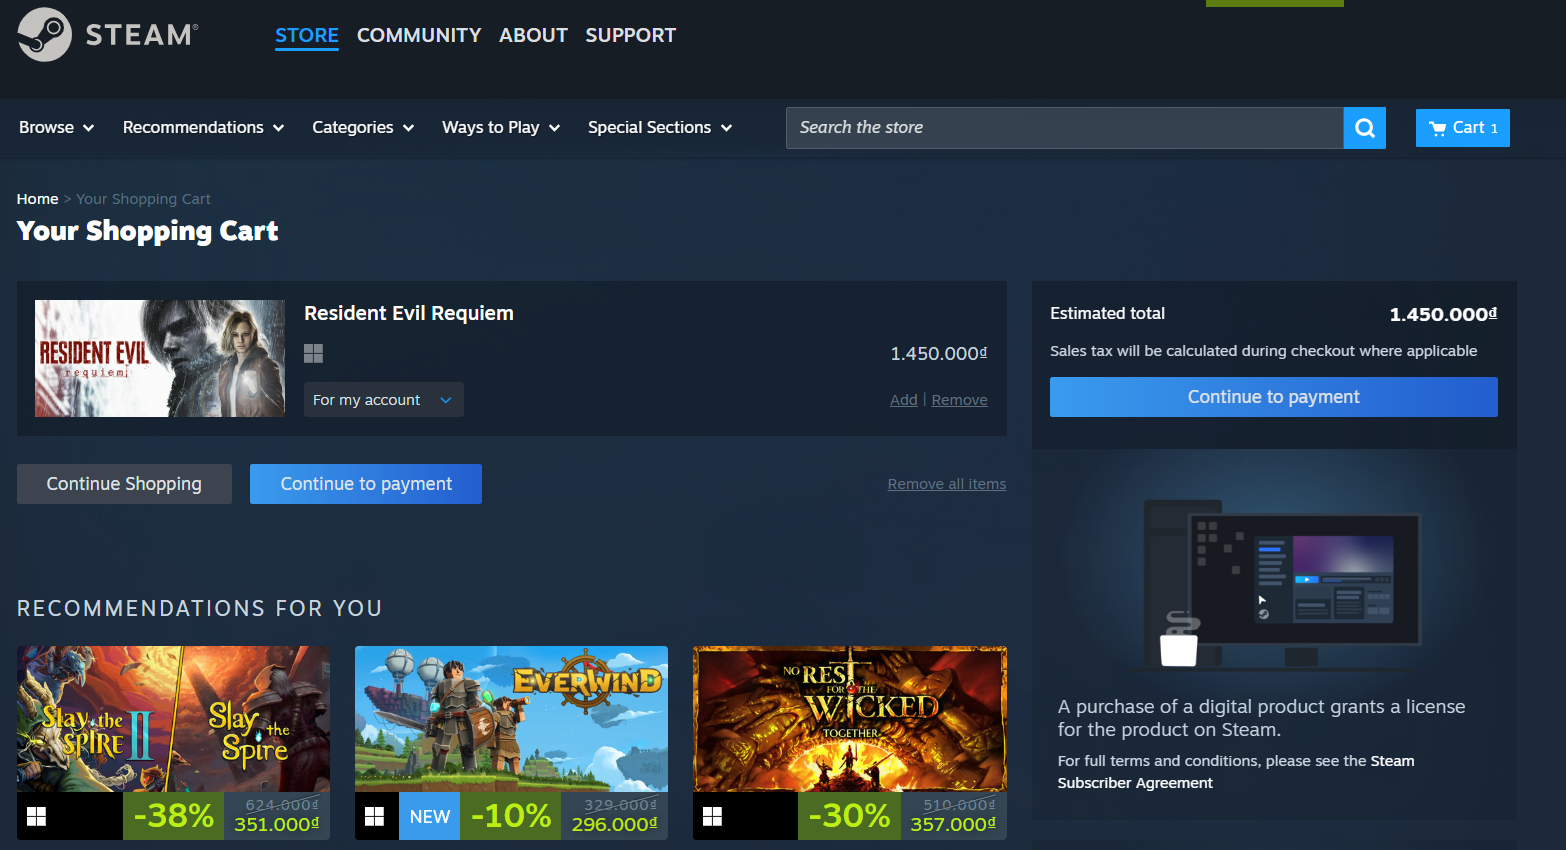
\includegraphics[width=0.6\linewidth]{graphics/steamcart.png}
    \caption{Steam shopping cart interface}
    \label{fig:steam_cart}
    
    \vspace{0.5em}
    {\raggedright
    \textit{This interface shows that Steam manages temporary purchase intent through a shopping cart before the checkout stage. It also presents pricing information, selected items, and a transition to payment, indicating that cart handling and transaction confirmation are treated as separate stages in the purchasing workflow.}
    \par}
\end{figure}
\paragraph{Ownership Management and Personal Library After Purchase}
A key business characteristic of Steam is that the user experience does not end once a purchase is completed. After a transaction is finalized, the purchased game is added to the player's personal library, where it remains accessible for future installation, play, and management. This shows that the platform does not treat a purchase as an isolated commercial event, but as the beginning of a longer-term ownership relationship between the player and the digital product.

From a system perspective, the transaction record and the personal library serve different business purposes:
\begin{itemize}
    \item the transaction records the commercial event at a specific point in time
    \item the library represents the player's ongoing ownership of digital content
\end{itemize}
This distinction is important because it implies that post-purchase data must be managed separately from purchase data. The library allows the platform to keep track of owned games over time and to support later interactions such as installation, playtime tracking, and access to related content. As a result, Steam demonstrates that digital ownership is not limited to payment confirmation, but extends into a persistent data relationship between the player and the purchased game.
From a business analysis perspective, this structure provides a strong foundation for the proposed system. It suggests that ownership-related data should be modeled independently from transaction data, while still remaining linked to the purchasing process. Therefore, Steam serves as a useful reference for understanding how digital products can move from purchase to long-term library management within an integrated platform.
\begin{figure}[h!]
    \centering
    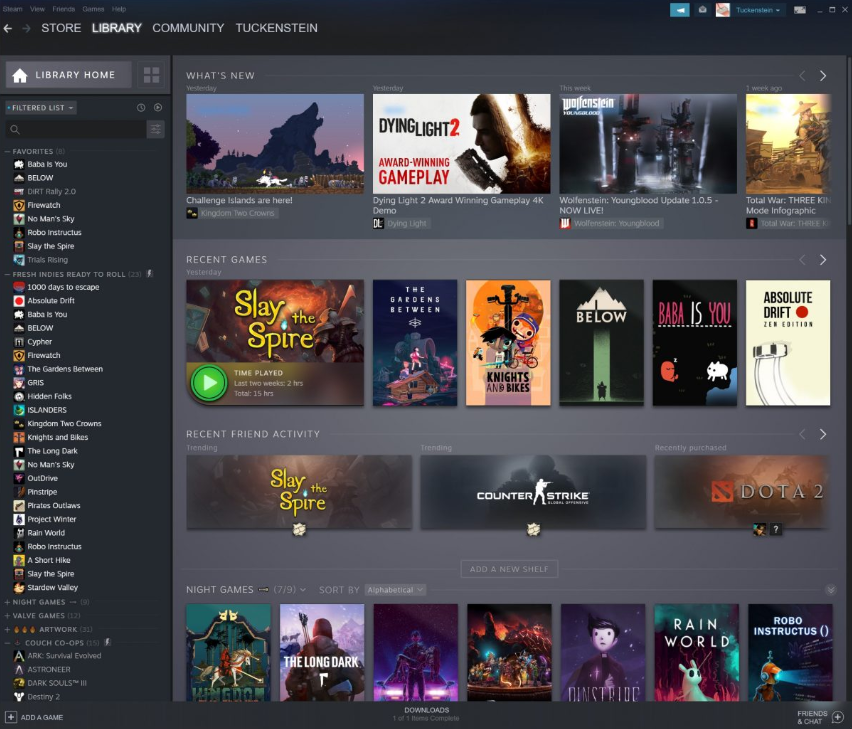
\includegraphics[width=0.6\linewidth]{graphics/libary1.png}
    \caption{Steam personal library interface}
    \label{fig:steam_cart}
    
    \vspace{0.5em}
    {\raggedright
    \textit{The personal library interface shows that purchased games are managed as persistent owned content after the transaction has been completed. This indicates that Steam treats digital ownership as an ongoing relationship between the player and the game rather than a one-time purchase event.}
    \par}
\end{figure}
\paragraph{Achievements, Engagement, and Post-Usage Data}
Steam also shows that the relationship between the player and the game continues after ownership has been established. Once a game is available in the personal library, the platform can track post-usage data that reflects how the player interacts with the product over time. This includes indicators such as playtime, recent activity, and achievement progress. Such data shows that Steam manages not only digital ownership, but also the player's ongoing engagement with purchased content.

From a business perspective, post-usage data serves several important functions:
\begin{itemize}
    \item it reflects the player's level of interaction with a game
    \item it supports personalized feedback and progress tracking
    \item it strengthens long-term engagement with the platform
\end{itemize}

Among these elements, achievements are especially significant because they represent specific milestones or goals associated with individual games. Their existence implies that the system must track not only which achievements belong to a game, but also which achievements have been unlocked by each player and when this occurred. This shows that Steam maintains gameplay-related records beyond the original purchase and library ownership data.

From a system analysis perspective, this observed structure provides a strong basis for the proposed system. It suggests that engagement-related data should be modeled separately from both transaction data and basic ownership data, while still remaining connected to the player and the game. Therefore, Steam serves as a useful reference for understanding how a digital platform can manage long-term user interaction, progress, and achievement-related information after purchase.
\begin{figure}[h!]
    \centering
    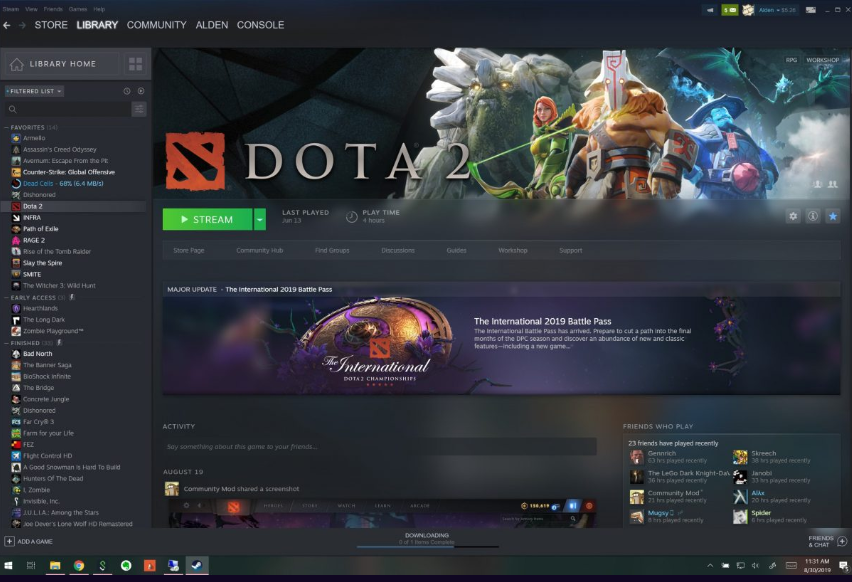
\includegraphics[width=0.75\linewidth]{graphics/library2.png}
    \caption{Steam game page within the personal library}
    \label{fig:steam_cart}
    
    \vspace{0.5em}
    {\raggedright
    \textit{The interface shows that Steam records post-usage data such as playtime and activity after a game has been added to the user's library.}
    \par}
\end{figure}
\paragraph{Community Interaction and User-Generated Content}
Steam also functions as a community platform in which users do more than purchase and own games. Players can write reviews, express positive or negative opinions, participate in discussions, and interact with other users through community-related features. This shows that the platform manages not only system-generated and publisher-provided data, but also user-generated content that contributes to how games are evaluated and discovered.

From a business perspective, community interaction adds value to the platform in several ways:
\begin{itemize}
    \item it allows users to share feedback and opinions about games
    \item it supports social participation beyond purchasing activities
    \item it influences how other users perceive and discover content
\end{itemize}

Among these elements, reviews are especially important because they connect a player directly to a specific game through rating behavior and written feedback. This implies that the system must manage review-related data such as the review content, recommendation outcome, and review date. More broadly, community functions show that Steam treats user participation as an important part of the platform rather than as a secondary feature.

From a system analysis perspective, this observed structure provides a strong basis for the proposed system. It suggests that community-related data should be modeled separately from transaction and ownership data, while still remaining connected to the player and the game. Therefore, Steam serves as a useful reference for understanding how a digital platform can manage user-generated content and social interaction alongside commercial functions.
\begin{figure}[h!]
    \centering
    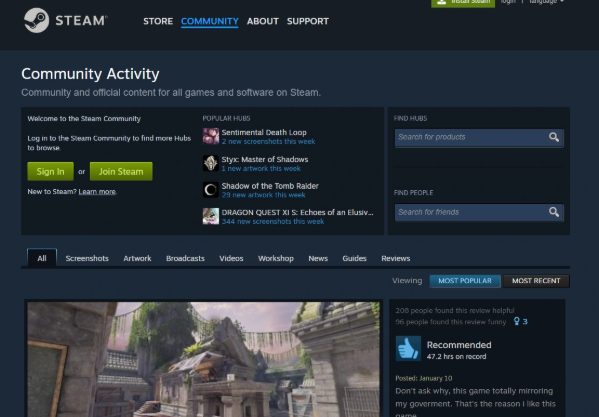
\includegraphics[width=0.75\linewidth]{graphics/community.png}
    \caption{Steam community interface}
    \label{fig:steam_cart}
    
    \vspace{0.5em}
    {\raggedright
    \textit{This interface shows that Steam supports community participation through reviews, hubs, and user-generated content such as screenshots and artwork. This indicates that the platform manages social interaction alongside its commercial functions.}
    \par}
\end{figure}
\paragraph{Developer/Publisher Participation and Content Lifecycle}
Steam also reflects the participation of developer and publisher-side actors through the way games are presented, updated, and commercially managed on the platform. Public product pages show developer and publisher information, release details, downloadable content, and promotional structures. This indicates that Steam supports not only consumer-side activities, but also the ongoing lifecycle management of digital products after their initial release.

From a business perspective, developer/publisher participation is important because it connects content creation with platform distribution and long-term commercial activity:
\begin{itemize}
    \item developers and publishers provide games to the platform
    \item product information must be maintained and updated over time
    \item additional content such as DLC can extend the lifecycle of a game
    \item promotions and pricing changes can influence continued sales performance
\end{itemize}

This observed structure suggests that a game on Steam is not a static item, but a managed digital product that may continue evolving after release. New content, revised information, and promotional events all indicate that the platform must support publisher-side product maintenance in addition to player-side consumption. As a result, Steam demonstrates that digital distribution platforms must coordinate both the commercial and content lifecycle aspects of each product.

From a system analysis perspective, this provides a strong basis for the proposed system. It suggests that developer/publisher-related data should be modeled separately from player data, while still remaining connected to games and their ongoing lifecycle. Therefore, Steam serves as a useful reference for understanding how publisher-side participation, content extension, and commercial management can be integrated into a digital distribution platform.
\\
\\
\vspace{0.5em}
\noindent{\large\bfseries Summary Observation}\par\vspace{0.3em}
Overall, Steam reflects a two-sided digital platform in which players and developers/publishers are connected through account management, product presentation, purchasing, digital ownership, community participation, and post-release content management. These business functions form an integrated workflow that provides a strong reference foundation for the proposed system described in Section 1.2. Based on this business analysis, the group can identify the main entities, attributes, and relationships of the proposed platform, while the semantic constraints and business rules that cannot be 
fully represented in the EERD will be presented separately in Section 1.3.
\newpage